
\chapter{Conclusions}
\label{Chapter-Conclusions}
\lhead{Chapter 7. \emph{Conclusions}}

%Motivation
% From universalities abstract
The importance of the network architecture on the mechanical properties of biopolymers is often obscured by focussing on the properties of single-components. \cite{storm_nonlinear_2005}, demonstrated that the nonlinear response of a strained network can be explained taking into account the non-linear properties of single-biopolymer and assuming that the network architecture is isotropic and homogeneous. This bottom-up approach has proven successful for a wide range of biopolymers \cite{carrillo_nonlinear_2013}, but might not be enough to explain the detailed onset of strain-stiffening and the exponent of the non-linear response, as shown recently with other protein networks\cite{licup_stress_2015}. An alternative explanation to non-linear elasticity was given with the focus on network architecture in the material\cite{onck_alternative_2005}, pointing out that the fine-grain control of non-linear elasticity depended on single-biopolymer components, the linkage characteristics, and the geometry of the connections.

% In order to study and compare different network geometries, a graph representation of the network is suitable, taking advantage of methods utilized in the field of complex networks. With this approach we could also explore the mechanisms of network formation,
% and see if there are connections between similar statistical distributions of the graph and the similarities showed by protein and polysaccharide networks \cite{carrillo_nonlinear_2013}.

Non-affine deformations are at the core of explaining the complex behaviour of biopolymer network, but we were lacking methods to reliably gather the geometry of the networks that this work try to address. Affine regimes are proved capable to characterize the mechanical properties of bulk and dense materials, but in biology this is not always the case. Growing filament networks will always face a non-affine regime in their early stages for example, so the mechanisms of network formation can be enlightened with the tools developed.

%Chapter Wavelets/image-tools
We rely on 3D imaging, tomography or stack of images, to extract the network geometry more reliably than in 2D. We had provided lacking tools for image analysis in 3D in a high-performance computing language, and contributed them, fully tested and documented to the de-facto standard image analysis library ITK in \autoref{Chapter-Wavelets}.

% Chapter TEM-SAXS
Gathering the network structure from images requires that the information on them is reliable. We showed in \autoref{Chapter-TEMSAXS} that the artifacts introduced by sample preparation don't interfere with the network size we are interested in. We have done it comparing small-angle x-ray scattering (SAXS) --that doesn't require sample preparation-- with our images, obtaining that above small scales, and in the range of the network geometry we are interested in, the agreement between imaging and scattering is good, so the network architecture can be extracted with confidence.

% Chapter Image / Extraction
We pursue our task of extracting the network from images in \autoref{Chapter-Image}, using a pipeline of image analysis to denoise and binarize the original images. We then developed state-of-the-art algorithms taken from the digital topology community to skeletonize the image, being aware of not changing the topology of the original network in the process. With a thin-image and introducing the novelty tools in this area, we create a one-one map between the image and a spatial graph, connecting in this way the image analysis field with the area of complex networks. We are now capable of study and characterize our network of biopolymers with a wider range of tools.

We compute the degree, end-to-end node distances, contour lengths, angle, and director cosines of those angles to characterize our sample networks of different biopolymers, ranging from actin filaments, to polysaccharides, such as pectin and carrageenan. The statistical distributions of these properties show strong similarities between protein and polysaccharides networks, which would be further explored to see its connection with network formation.

% Chapter Reconstruction
We also provide a simulated annealing tool in \autoref{Chapter-Reconstruction} to recreate networks completely in-silico given a set of statistical distributions: degree, end-to-end distance, and director cosines. This allow the theoretical exploration of networks just changing the input distributions. Future work in this area might include adding distributions for others graph properties for finer control.


In conclusion, we have focused in bringing computation tools to the community (all the work is open source, tested and documented) where we can start investigating low density, non-affine networks from a more analytical point of view, I foresee theoreticians and modellers taking these networks extracted from experimental results as starting points for their models, instead of relying on the more homogeneous mikado model, and at a greater scale than lattice models.

\begin{figure}[h!]
  \begin{center}
    \begin{tikzpicture}[scale=0.8]
      \node[blockimage] (A) at (2,8.5) {
      \textsc{Image Analysis}};
      \node[blocknetwork] (B) at (8.5,3) {%
        \begin{center}
        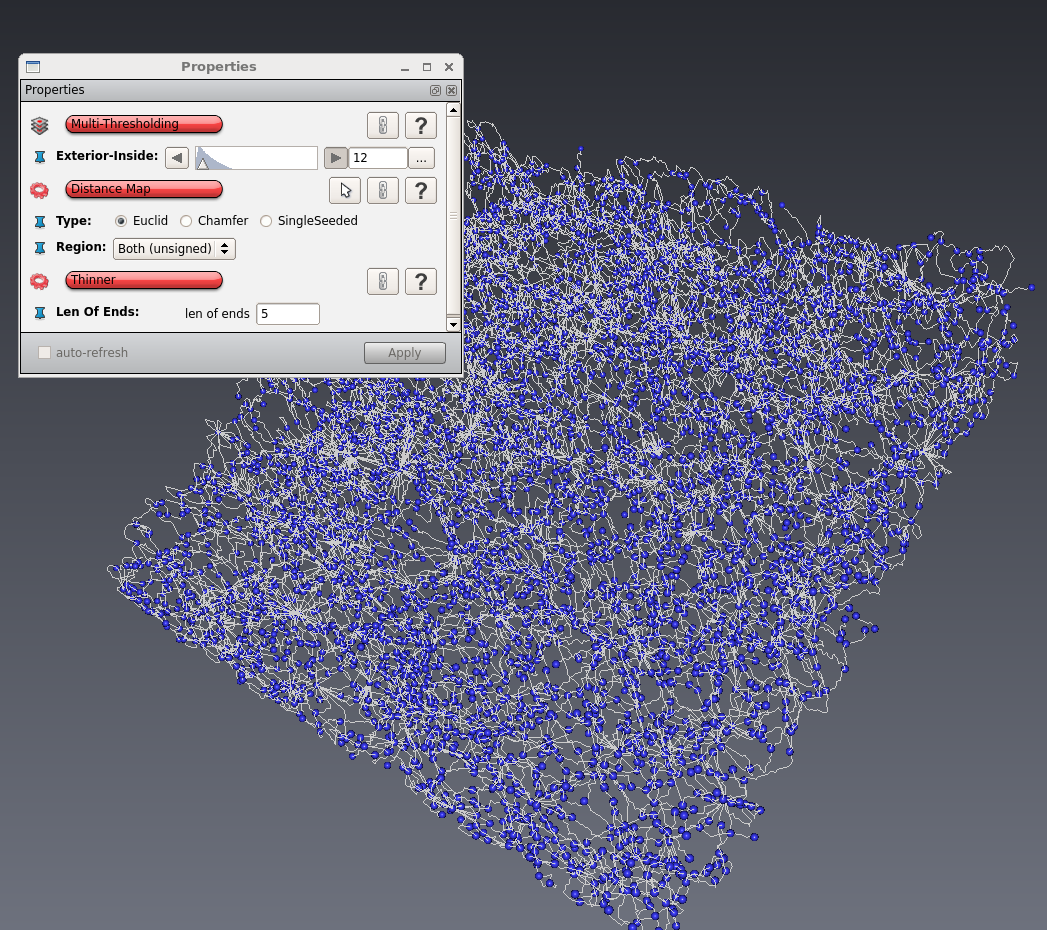
\includegraphics[width=1.0\textwidth]{Figures/chapter-image/avizo/ActinAllan11jun132_BIN12LEN5.png}%
        \end{center}

       \textsc{Network /}\\
       \textsc{Spatial Graph}
        };

      \node[blockimage] (C) at (1.5,0) {
      \textsc{Reconstruction}\\
      \textsc{Algorithm}
      };
      \node[blocknetwork] (F) at (0,3.5) {
      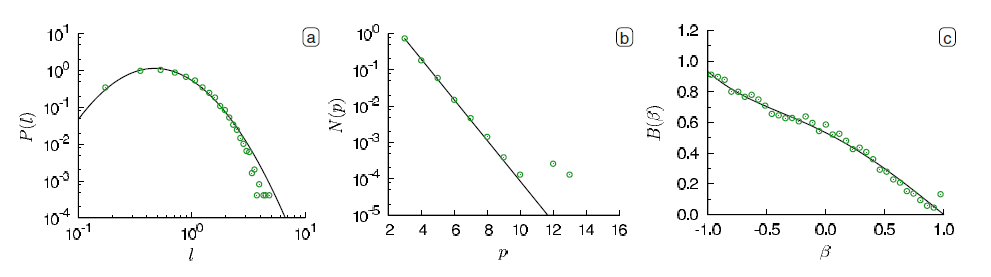
\includegraphics[width=1.0\textwidth]{Figures/chapter-reconstruct/lindstrom-paper-images.png}%

      \textsc{Statistics}
      };

      \node[blockmodel] (D) at (15,3) {\textsc{Modeling}}; 

      \draw[green,arrows={-triangle 45}] (A) -- (B);
      \draw[blue,arrows={-triangle 45}] (B) -- (F);
      \draw[blue,arrows={-triangle 45}] (F) -- (C);
      \draw[red,arrows={-triangle 45}] (B) -- (D);
      \draw[green,arrows={-triangle 45}] (C) -- (B);

    \end{tikzpicture}
  \end{center}
  \caption[Scheme of the thesis]{Scheme of the project. }
\end{figure}

% \subsection{Future Work}%
% \label{sub:future_work}




